%==============================================================================
% Chapitre 64 - Lecture des désignations commerciales
%==============================================================================

\section{Introduction}

Les boîtes de cartouches comportent de nombreuses informations destinées à
identifier les caractéristiques principales des munitions.

La compréhension de ces indications facilite le choix d'un chargement adapté à
l'usage recherché.

\begin{aretenir}

Les désignations commerciales résument plusieurs caractéristiques importantes
de la cartouche.

\end{aretenir}

\section{Pourquoi autant d'informations ?}

Une cartouche de chasse peut être décrite par de nombreux paramètres :

\begin{itemize}
    \item calibre ;
    \item longueur ;
    \item masse de charge ;
    \item type de projectile ;
    \item matériau ;
    \item vitesse annoncée.
\end{itemize}

Les fabricants regroupent généralement ces informations sur l'emballage.

\begin{figure}[htbp]
\centering

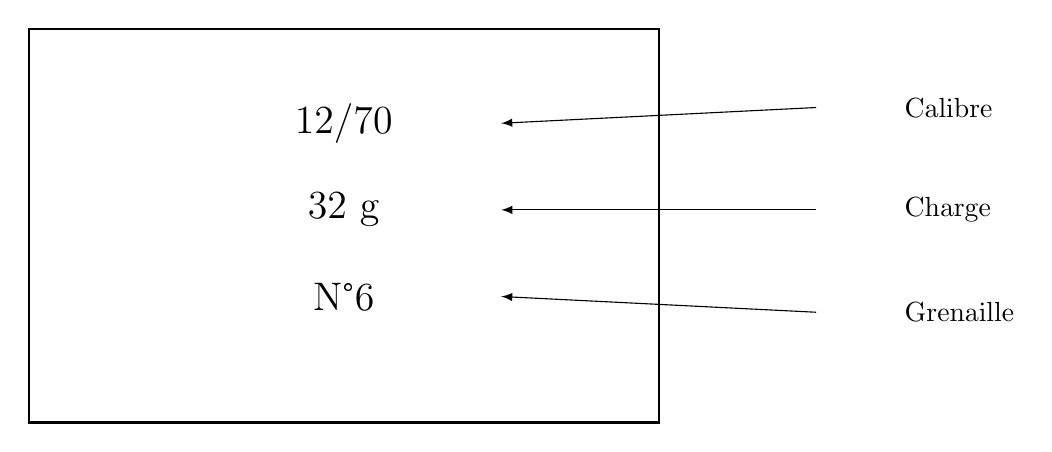
\begin{tikzpicture}

% Boîte
\draw[thick]
(0,0)
rectangle
(8,5);

\node[font=\Large]
at (4,3.8)
{12/70};

\node[font=\Large]
at (4,2.7)
{32 g};

\node[font=\Large]
at (4,1.6)
{N°6};

% Flèches
\node[right]
at (11,4)
{Calibre};

\draw[-latex]
(10,4)
--
(6,3.8);

\node[right]
at (11,2.7)
{Charge};

\draw[-latex]
(10,2.7)
--
(6,2.7);

\node[right]
at (11,1.4)
{Grenaille};

\draw[-latex]
(10,1.4)
--
(6,1.6);

\end{tikzpicture}

\caption{Exemple simplifié des informations visibles sur une boîte de cartouches.}
\label{fig:boite_cartouches}

\end{figure}


\section{Le calibre}

Le calibre constitue souvent la première information visible.

Il indique la famille d'armes pour laquelle la cartouche est conçue.

\section{La longueur}

La longueur figure généralement à côté du calibre.

Par exemple :

\begin{quote}
12/70
\end{quote}

Cette notation combine le calibre et la longueur nominale de la cartouche.

\section{La masse de charge}

Les cartouches à grenaille indiquent fréquemment la masse totale de la charge.

Cette valeur est généralement exprimée en grammes.

\section{Le numéro de grenaille}

Le numéro de grenaille renseigne sur la taille des projectiles.

Cette information influence directement les performances attendues.

\section{Le matériau}

Le matériau utilisé peut également être indiqué :

\begin{itemize}
    \item plomb ;
    \item acier ;
    \item bismuth ;
    \item tungstène.
\end{itemize}

\section{La vitesse annoncée}

Certains fabricants communiquent une vitesse mesurée selon des conditions
déterminées.

Cette valeur permet de comparer différents chargements.

\section{Les appellations commerciales}

Les fabricants utilisent également des noms commerciaux destinés à identifier
certaines gammes de produits.

Ces appellations ne remplacent pas les caractéristiques techniques.

\begin{figure}[htbp]
\centering

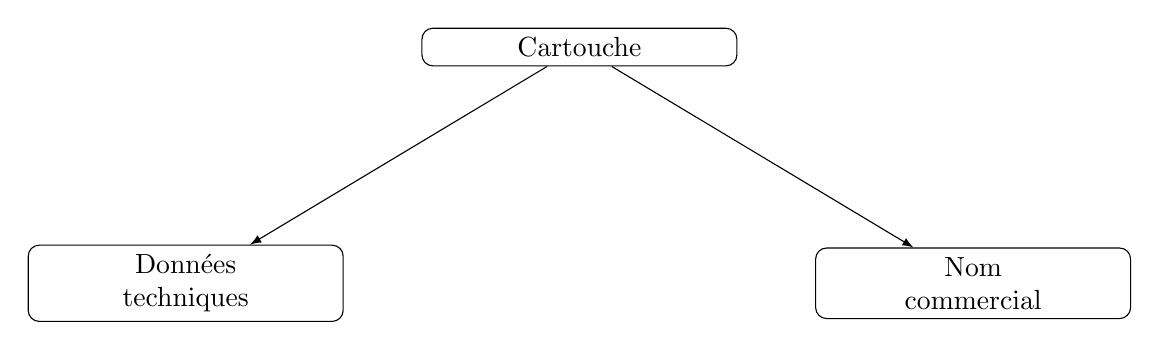
\begin{tikzpicture}[
every node/.style={
draw,
rounded corners,
align=center,
minimum width=4cm
}
]

\node (C)
at (0,0)
{Cartouche};

\node (T)
at (-5,-3)
{Données\\techniques};

\node (M)
at (5,-3)
{Nom\\commercial};

\draw[-latex]
(C)
--
(T);

\draw[-latex]
(C)
--
(M);

\end{tikzpicture}

\caption{Une cartouche est généralement identifiée à la fois par des données techniques et une appellation commerciale.}
\label{fig:technique_commercial}

\end{figure}

\section{Les marquages de sécurité}

Les emballages peuvent comporter des informations complémentaires relatives :

\begin{itemize}
    \item à la compatibilité ;
    \item à l'utilisation ;
    \item aux précautions d'emploi.
\end{itemize}

\section{Lecture complète d'un exemple}

Une désignation telle que :

\begin{quote}
12/70 -- 32 g -- N°6
\end{quote}

fournit déjà plusieurs informations importantes.

\begin{figure}[htbp]
\centering

\begin{tikzpicture}

\node[font=\Large]
(T)
at (0,0)
{12 / 70 -- 32 g -- N°6};

% Calibre
\draw[-latex]
(-1.9,-0.3)
--
(-5,-1.5);

\node[left]
at (-5,-1.5)
{Calibre};

% Longueur
\draw[-latex]
(-1.1,-0.3)
--
(-2,-2.2);

\node
at (-2,-2.8)
{Longueur};

% Charge
\draw[-latex]
(0.5,-0.3)
--
(0.7,-2.2);

\node
at (0.7,-2.8)
{Charge};

% Grenaille
\draw[-latex]
(1.8,-0.3)
--
(5,-1.5);

\node[right]
at (5,-1.5)
{Numéro de grenaille};

\end{tikzpicture}

\caption{Exemple de lecture d'une désignation commerciale.}
\label{fig:lecture_designation_complete}

\end{figure}

\section{Éviter les confusions}

Certaines désignations peuvent sembler proches.

Il est important de distinguer :

\begin{itemize}
    \item le calibre ;
    \item la longueur ;
    \item la masse de charge ;
    \item la taille des projectiles.
\end{itemize}

\section{Pourquoi comparer plusieurs paramètres ?}

Aucune caractéristique ne permet à elle seule d'évaluer complètement une
munition.

L'analyse doit prendre en compte l'ensemble des informations disponibles.

\section{Vers la synthèse des munitions de chasse}

Les chapitres précédents ont présenté les principaux composants, projectiles
et chargements utilisés dans les fusils de chasse.

Le chapitre suivant proposera une synthèse générale avant d'aborder la
balistique intérieure.

\section{À retenir}

\begin{aretenir}

\begin{itemize}
    \item Les désignations commerciales regroupent plusieurs informations.
    \item Le calibre et la longueur constituent des indications essentielles.
    \item La masse de charge et le numéro de grenaille influencent les
          performances.
    \item Les appellations commerciales complètent les données techniques.
    \item Une lecture correcte évite de nombreuses erreurs.
\end{itemize}

\end{aretenir}

\begin{figure}[htbp]
\centering

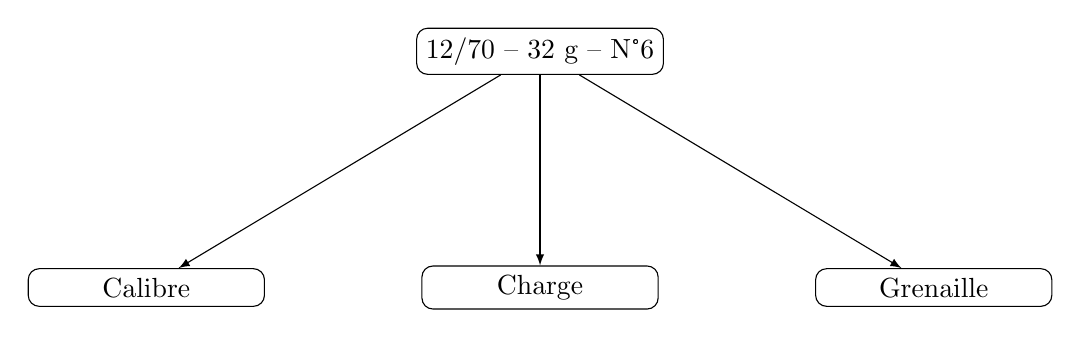
\begin{tikzpicture}[
every node/.style={
draw,
rounded corners,
align=center,
minimum width=3cm
}
]

\node (D)
at (0,0)
{12/70 -- 32 g -- N°6};

\node (C)
at (-5,-3)
{Calibre};

\node (L)
at (0,-3)
{Charge};

\node (G)
at (5,-3)
{Grenaille};

\draw[-latex] (D) -- (C);
\draw[-latex] (D) -- (L);
\draw[-latex] (D) -- (G);

\end{tikzpicture}

\caption{Les principales informations contenues dans une désignation commerciale.}
\label{fig:hierarchie_designation}

\end{figure}
